\documentclass[aspectratio=169,hyperref={pdfpagelabels=false}]{beamer}
\usepackage{helvet}
\usepackage[english]{babel}
\usepackage{pgfplots}
\usepackage{pgf}
\pgfplotsset{compat=newest}
\usepackage{booktabs}
\usepackage[T1]{fontenc}
\usepackage[utf8]{inputenc}
\usepackage{lipsum}
\usepackage{tcolorbox}
\usepackage{xcolor}
\usepackage{listings}
\usepackage{microtype}
\usepackage{float}
\usepackage{siunitx}
\usepackage{multicol}
\usepackage{hyperref}
\usepackage{dsfont}
\usepackage{caption}
\usepackage{subcaption}

% DTU colours for diagrams
% You might want to make the front/back page background colour the first colour in the plot cycle list.
\pgfplotscreateplotcyclelist{DTU}{%
dtured,         fill=dtured,        \\%
blue,           fill=blue,          \\%
brightgreen,    fill=brightgreen    \\%
navyblue,       fill=navyblue       \\%
yellow,         fill=yellow         \\%
orange,         fill=orange         \\%
grey,           fill=grey           \\%
red,            fill=red            \\%
green,          fill=green          \\%
purple,         fill=purple         \\%
}

% Table of contents (TOC) and numbering of headings
\setcounter{tocdepth}{1}    % Depth of table of content: sub sections will not be included in table of contents
\setcounter{secnumdepth}{2} % Depth of section numbering: sub sub sections are not numbered



\newcommand{\setcolor}[1]{\def\chosencolor{#1}}
\newcommand{\setdepartment}[1]{\def\department{#1}}

\usetheme{DTU}
\setbeamersize{text margin left=22mm}
\def\insertframetitle{}

\newcommand{\inserttitlepage}{
    \begin{frame}[plain, noframenumbering]{}

        \begin{center}
        \hspace{-3.6em}
            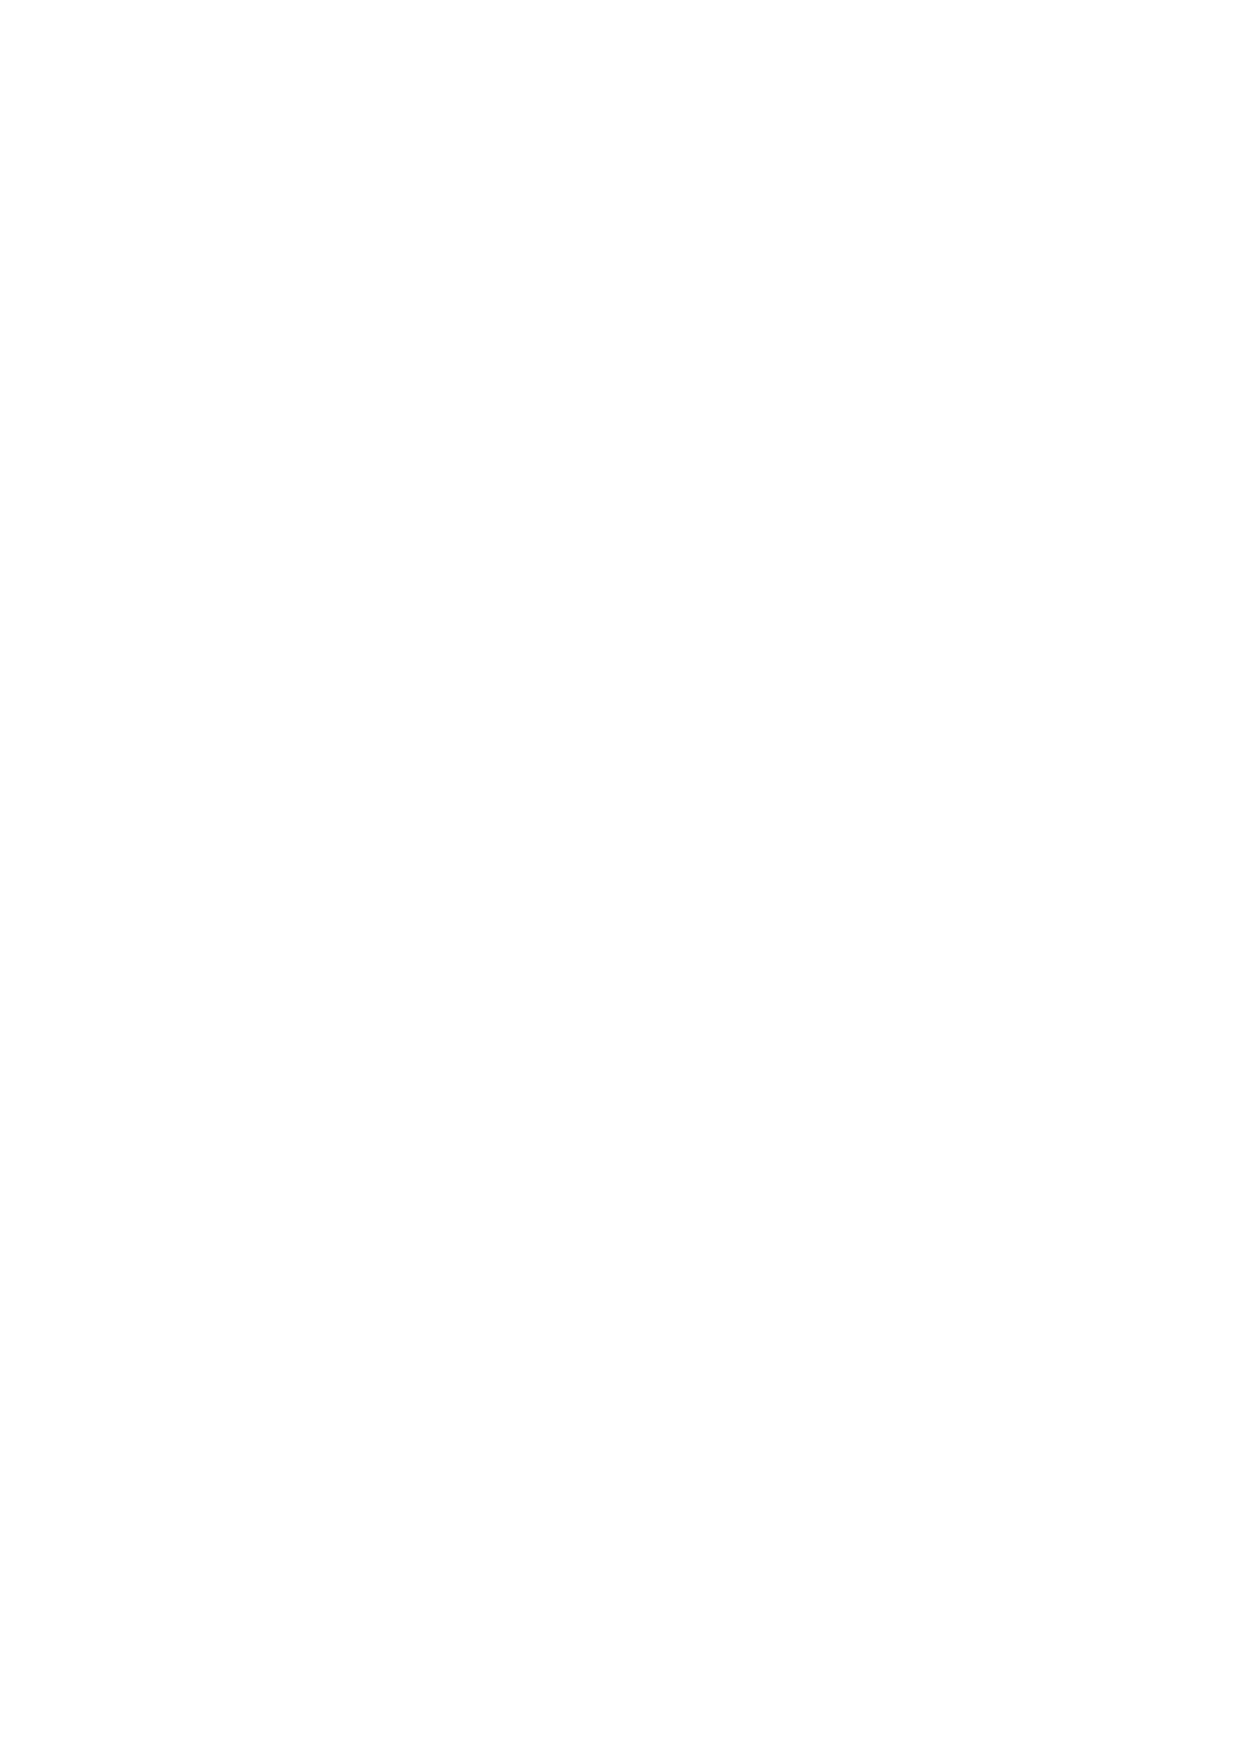
\includegraphics[width = 0.25\paperwidth]{logos/\targetcolourmodel/white.pdf}
        \end{center}
        
    \end{frame}

    \begin{frame}[plain]{}
        \color{white}\maketitle    
    \end{frame}

    \setbeamercolor{background canvas}{bg = white}
}



\subtitle{Gustav Lang Moesmand}
\title{Computer Vision Exam Slides}

\setdepartment{DTU Compute}
\setcolor{green}



\begin{document}
\inserttitlepage

\begin{frame}{ Week 1: Homogeneous coordinates and pinhole model }
\begin{columns}
	\begin{column}{.3\textwidth}
		\begin{block}{box3d(n)}
			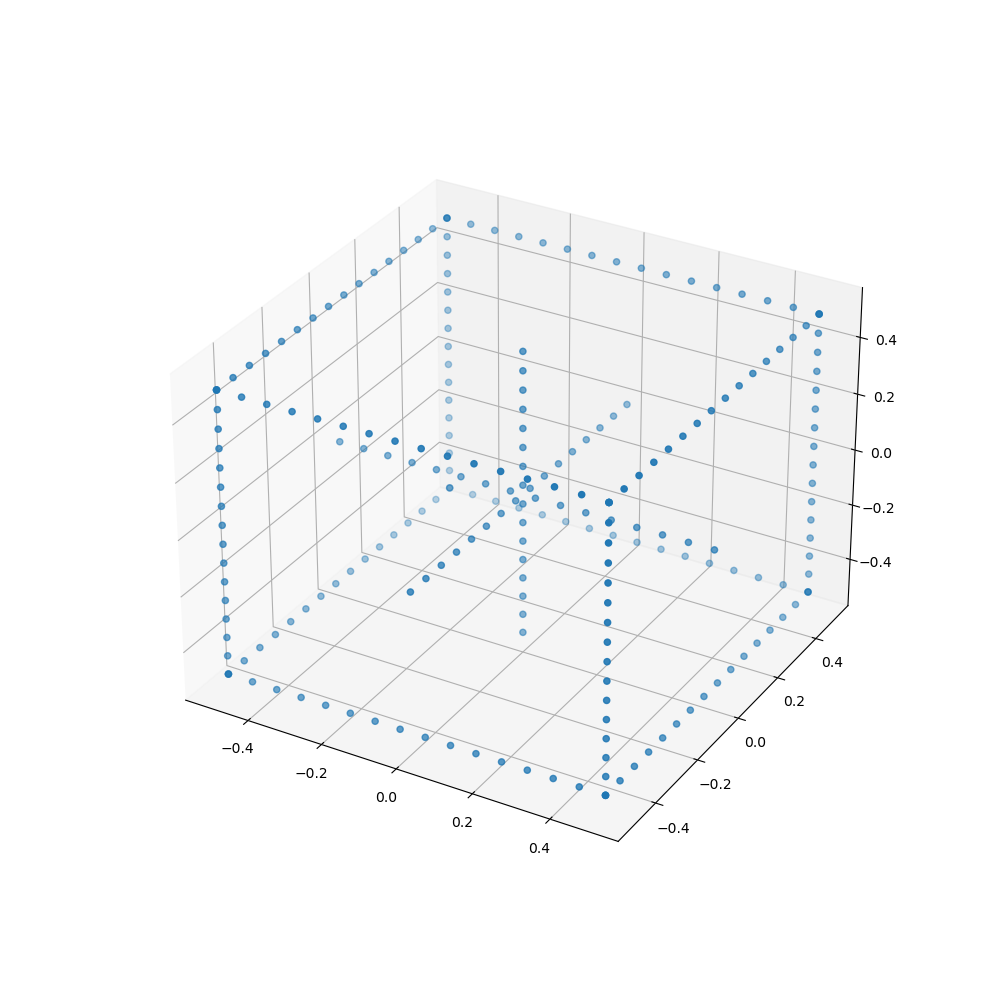
\includegraphics[width=\textwidth]{exercise_imgs/ex1-11.png}
		\end{block}					
	\end{column}	
	\begin{column}{.3\textwidth}
		\begin{block}{Project points}
			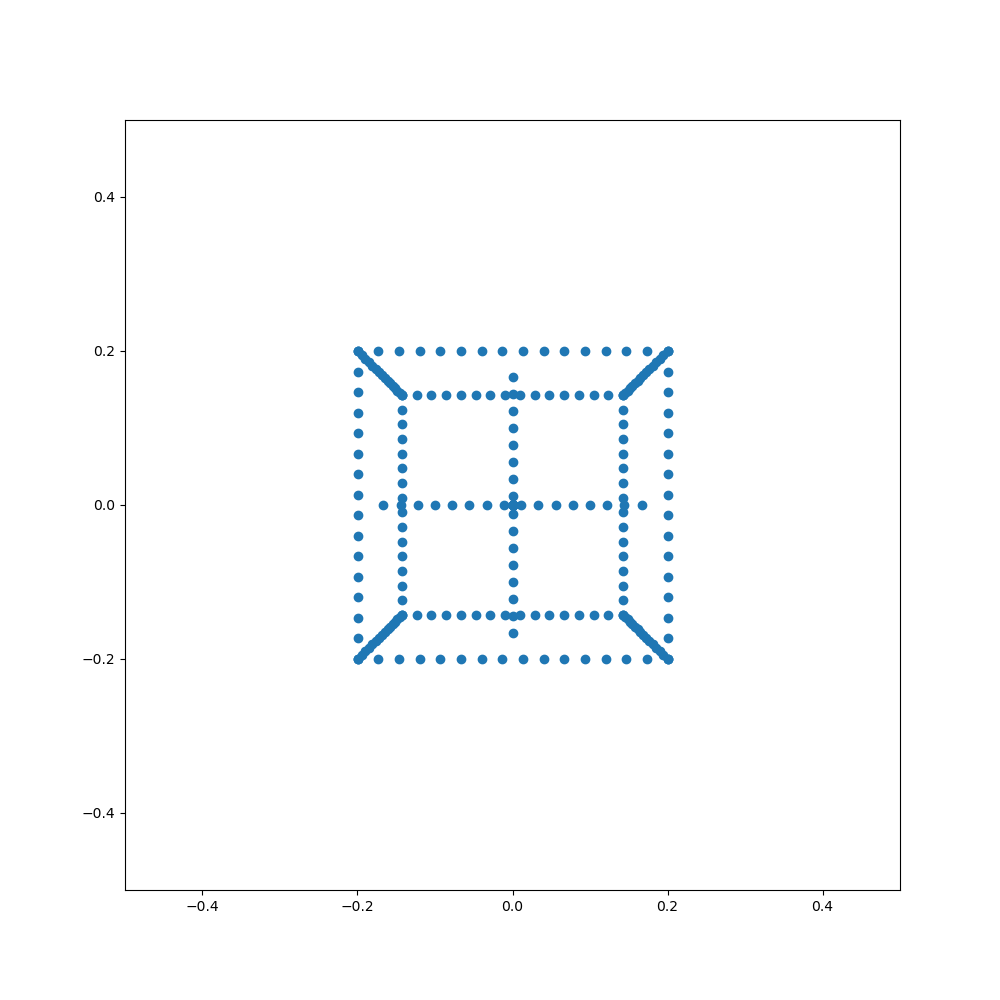
\includegraphics[width=\textwidth]{exercise_imgs/ex1-12.png}
		\end{block}					
	\end{column}	
	\begin{column}{.3\textwidth}
		\begin{block}{Projection with rotation}
			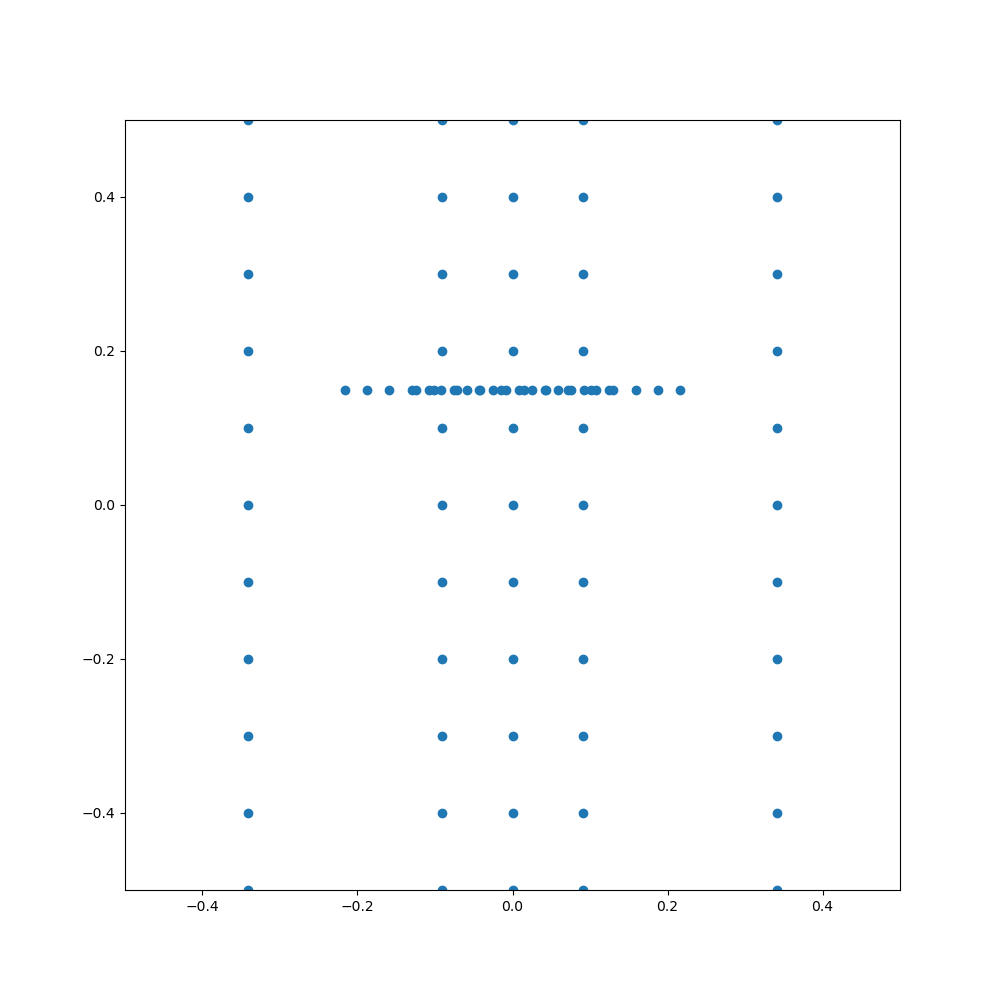
\includegraphics[width=\textwidth]{exercise_imgs/ex1-13.png}
		\end{block}					
	\end{column}	
\end{columns}	
\end{frame}

\begin{frame}{ Week 2: Camera model and homographies }
\begin{columns}
	\begin{column}{.3\textwidth}
		\begin{block}{$\delta r(r) = -0.2^2$}
			\begin{center}
				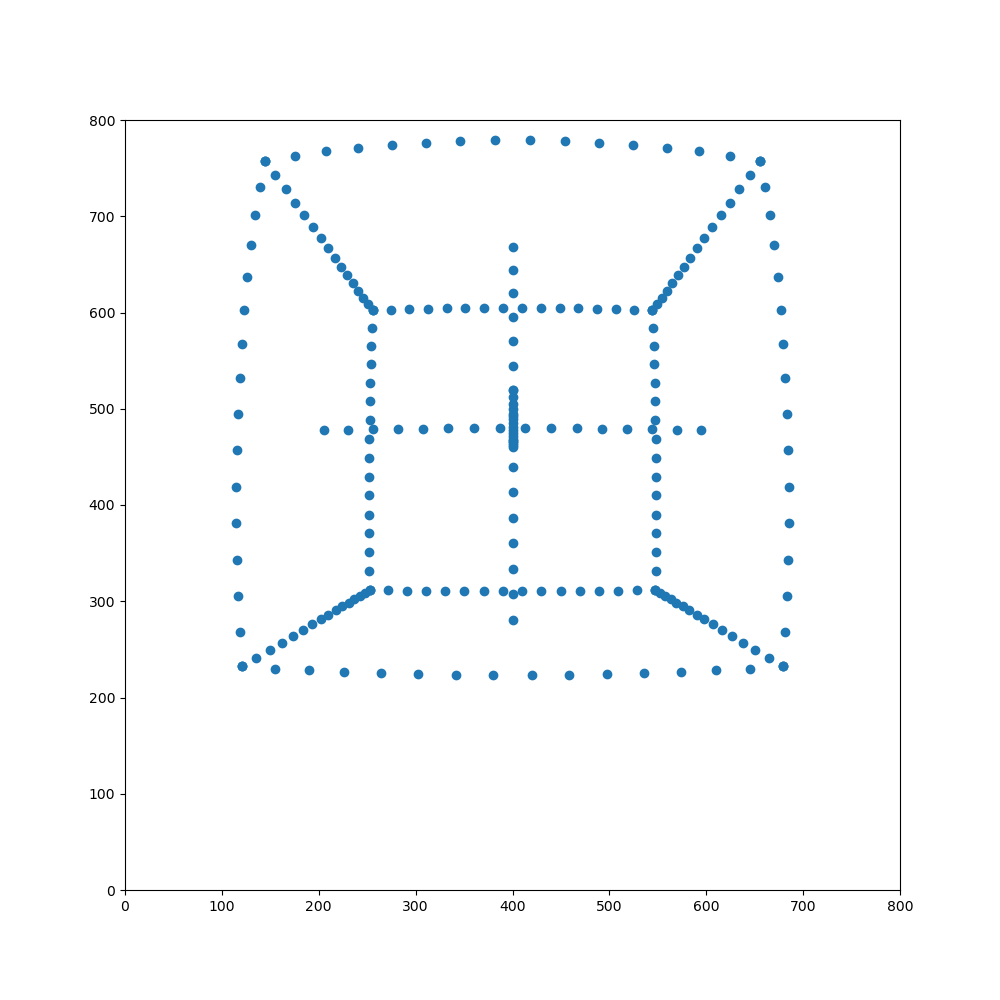
\includegraphics[width=1\textwidth]{exercise_imgs/ex2-2.png}
			\end{center}
		\end{block}					
	\end{column}	
	\begin{column}{.7\textwidth}
		\begin{block}{Straigtened image}
			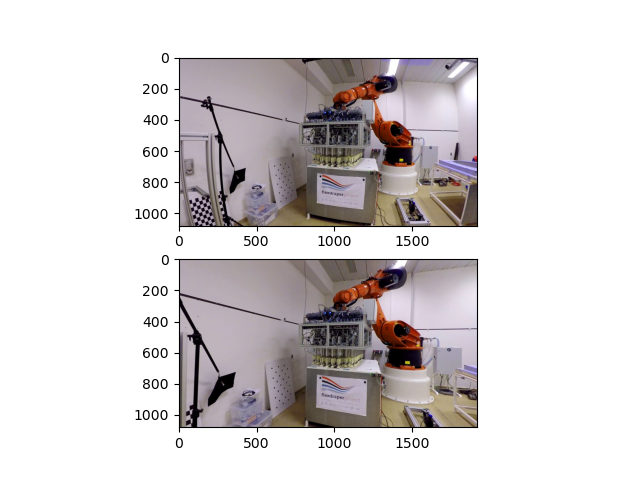
\includegraphics[width=\textwidth]{exercise_imgs/ex2-4.png}
		\end{block}					
	\end{column}	
\end{columns}	

\end{frame}

\begin{frame}{ Week 3: Multi-view geometry }
\begin{columns}
	\begin{column}{.5\textwidth}
		\begin{block}{Images side by side}
			\begin{center}
				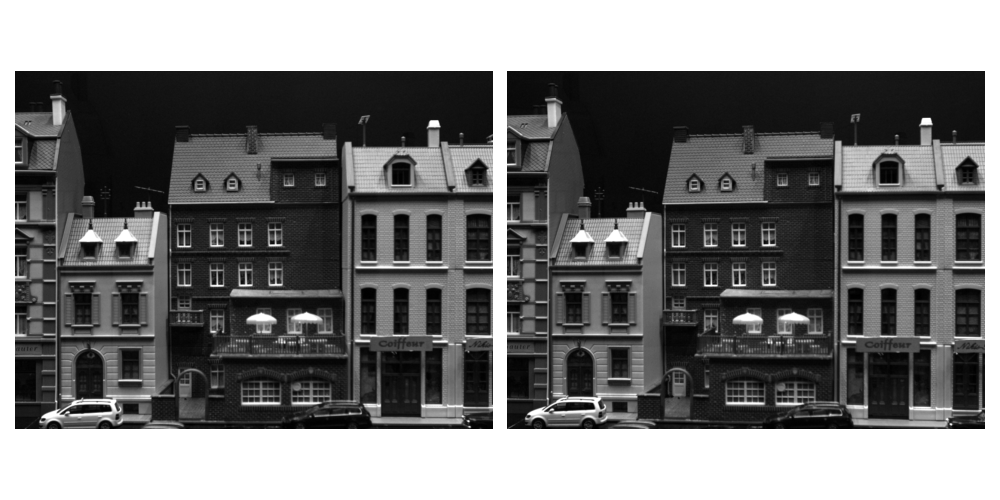
\includegraphics[width=\textwidth]{exercise_imgs/ex3-8.png}
			\end{center}
		\end{block}					
	\end{column}	
	\begin{column}{.5\textwidth}
		\begin{block}{Epipolar point to line}
		\begin{center}
			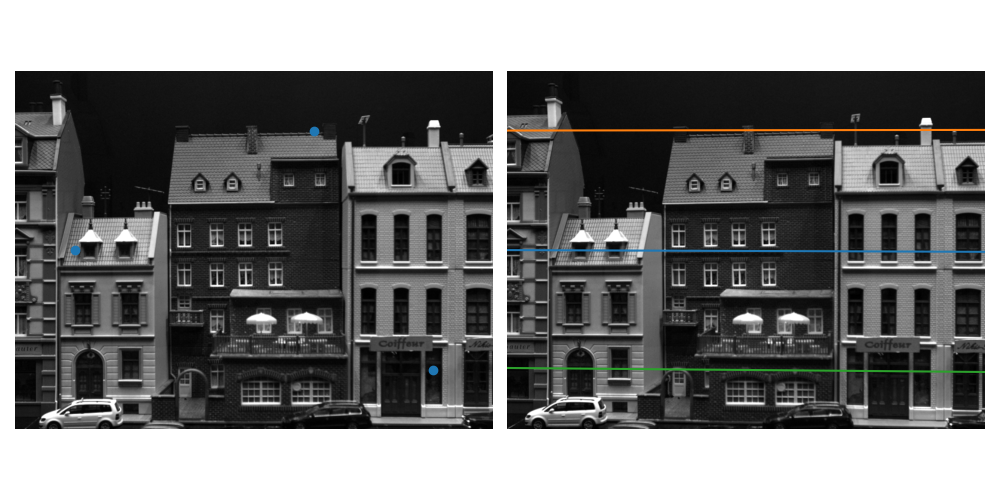
\includegraphics[width=\textwidth]{exercise_imgs/ex3-9.png}
		\end{center}
		\end{block}					
	\end{column}	
\end{columns}	

\end{frame}

\begin{frame}{ Week 4: Camera calibration }
\begin{columns}
	\begin{column}{.5\textwidth}
		\begin{block}{Rotated checkerboard points}
			\begin{center}
				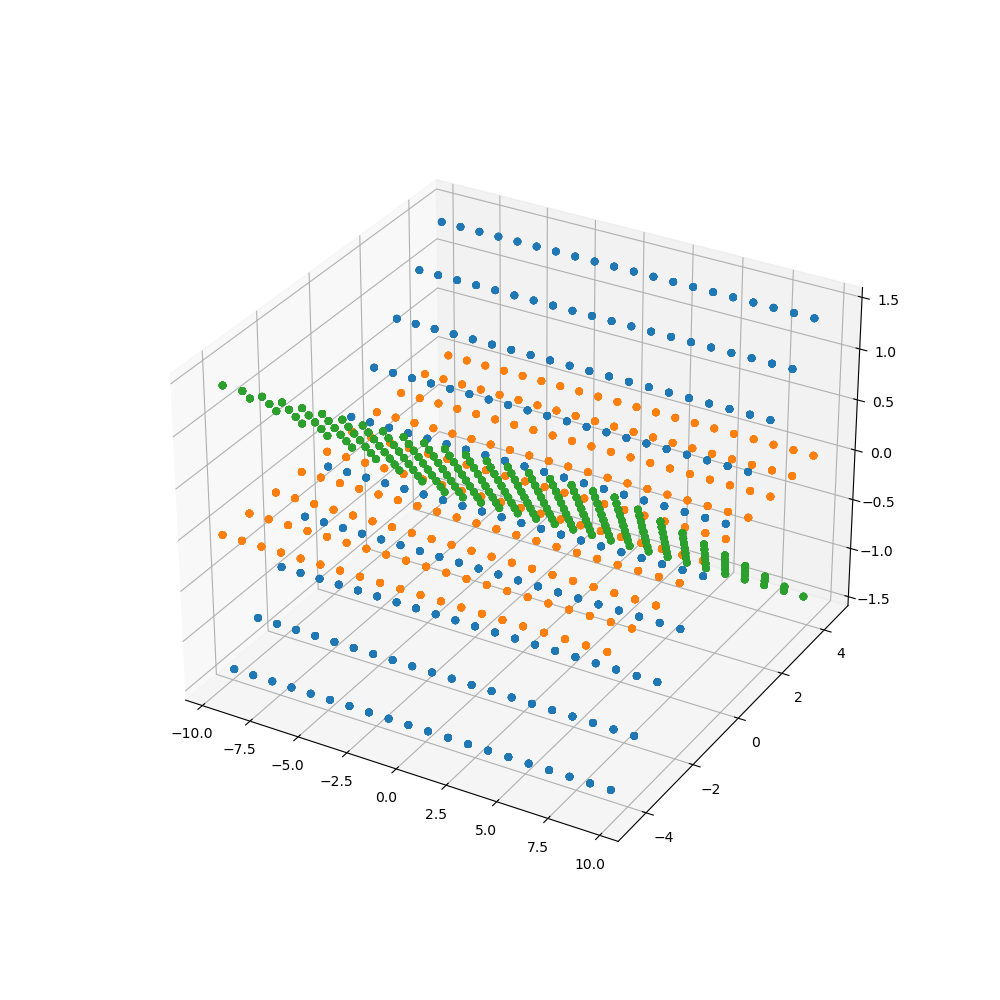
\includegraphics[width=\textwidth]{exercise_imgs/ex4-4-1.png}
			\end{center}
		\end{block}					
	\end{column}	
	\begin{column}{.5\textwidth}
		\begin{block}{As seen from image plane}
		\begin{center}
			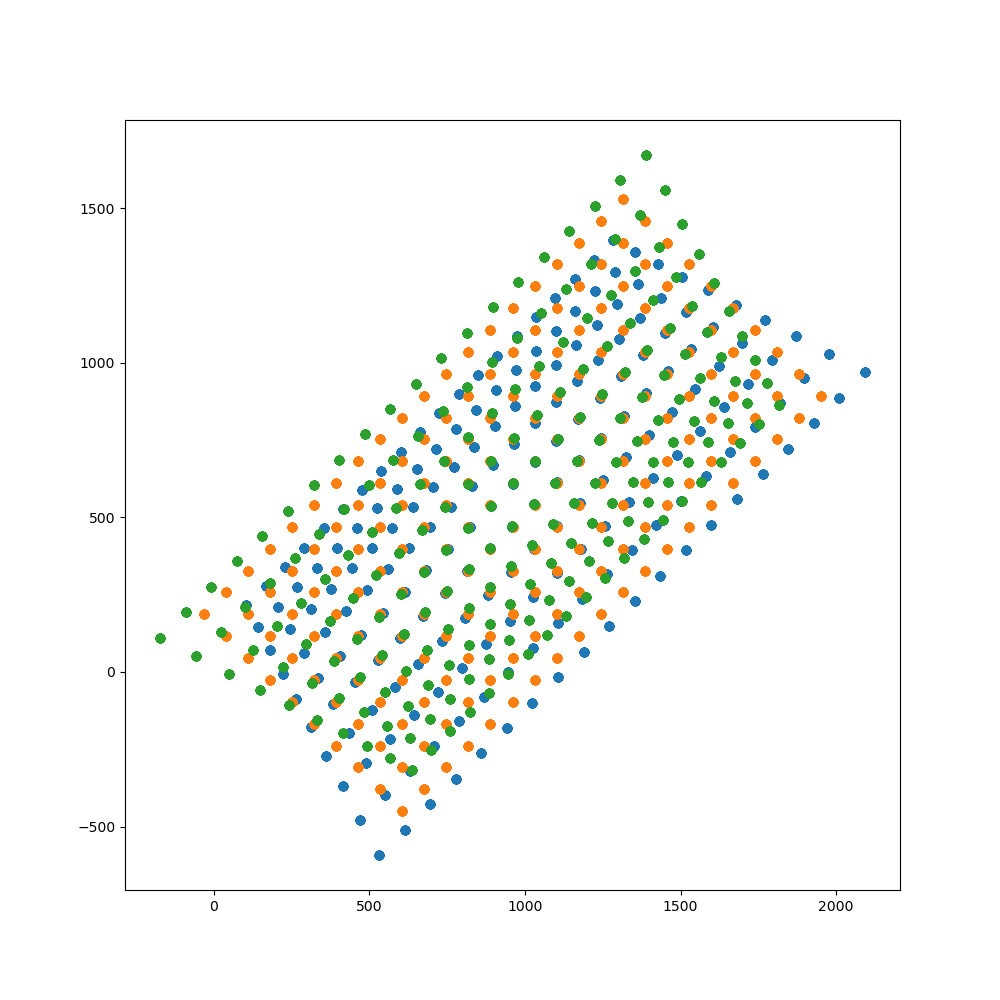
\includegraphics[width=\textwidth]{exercise_imgs/ex4-4-2.png}
		\end{center}
		\end{block}					
	\end{column}	
\end{columns}	
\end{frame}

\begin{frame}{ Week 5: Nonlinear optimization and camera calibration }
	\begin{block}{Reprojected checkerboard points, total pixel error shown as title}
		\begin{center}	
			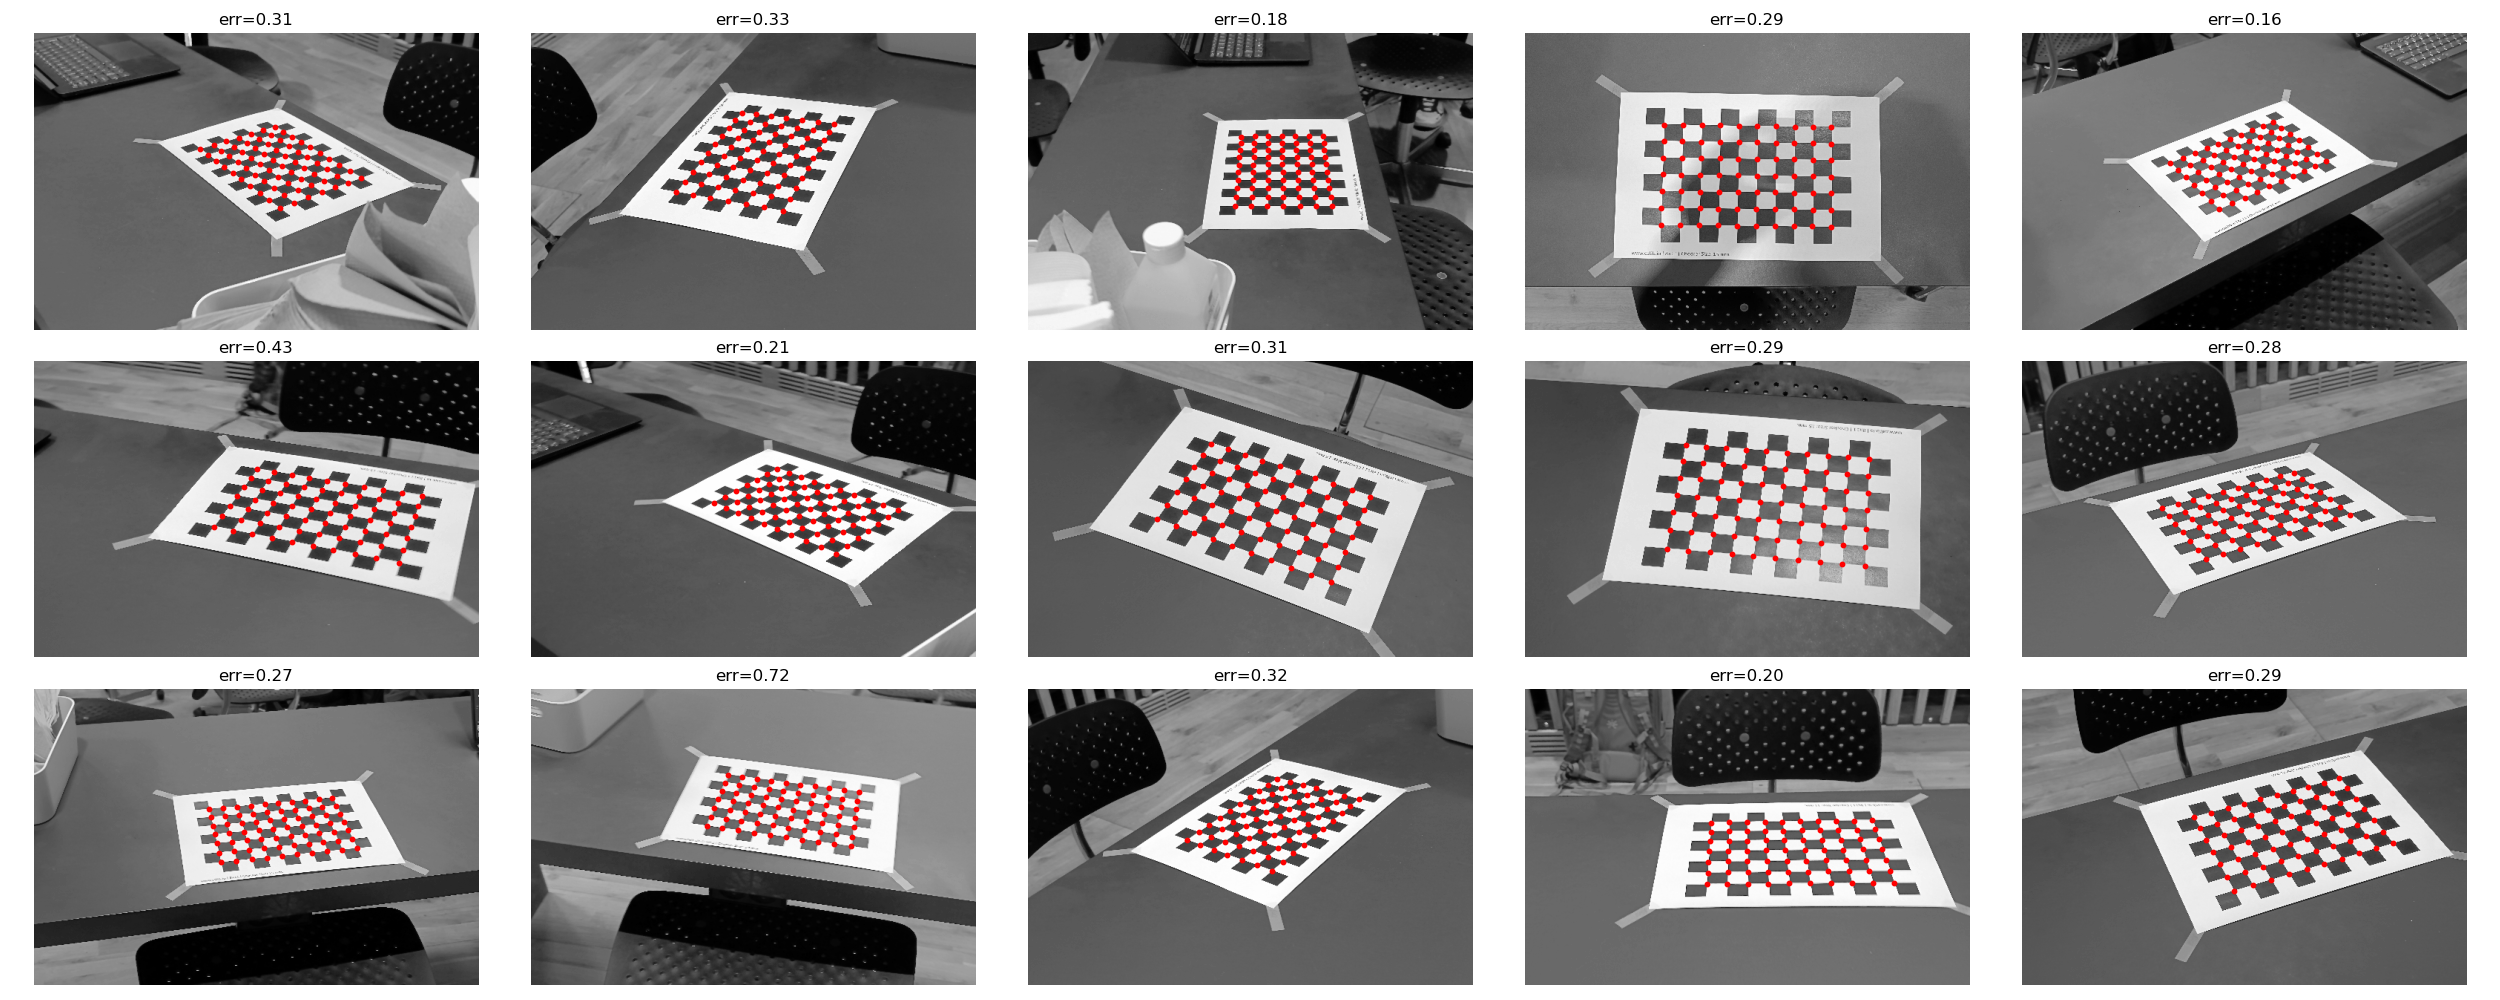
\includegraphics[width=\textwidth]{exercise_imgs/ex5-8.png}
		\end{center}
	\end{block}
\end{frame}

\begin{frame}{ Week 6: Simple features }
	\begin{columns}
		\begin{column}{.45\textwidth}
			\begin{block}{Harris corner detection}
			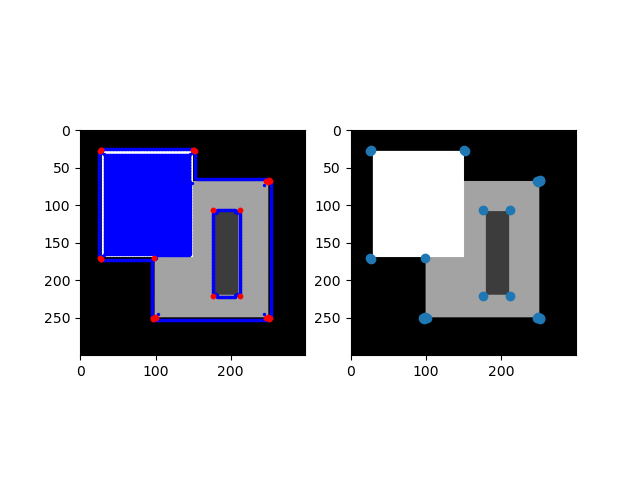
\includegraphics[width=\textwidth]{exercise_imgs/ex6-5.png}
			\end{block}
		\end{column}
		\begin{column}{.45\textwidth}
			\begin{block}{Canny edge detector}
			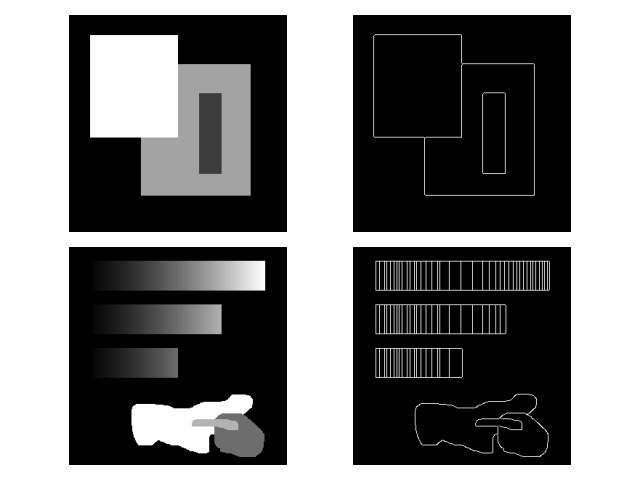
\includegraphics[width=\textwidth]{exercise_imgs/ex6-6.png}
			\end{block}
		\end{column}
	\end{columns}
\end{frame}

\begin{frame}{ Week 7: Robust model fitting }
	\begin{columns}
		\begin{column}{.45\textwidth}
			\begin{block}{RANSAC for estimating lines}
			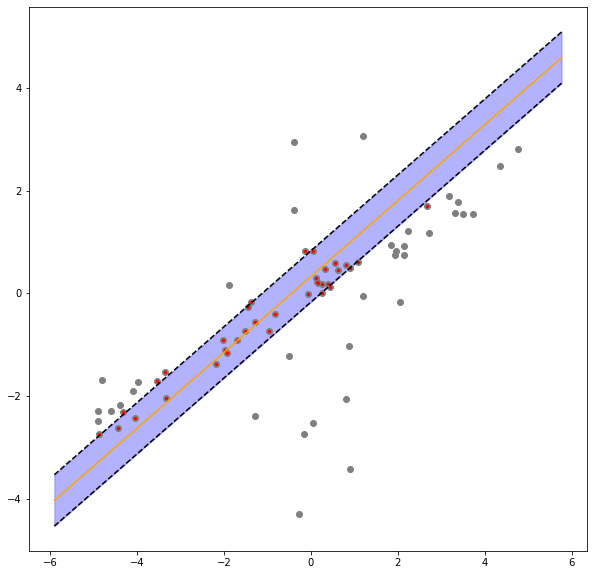
\includegraphics[width=\textwidth]{exercise_imgs/ex7-5.png}
			\end{block}
		\end{column}
		\begin{column}{.45\textwidth}
			\begin{block}{Line fitted to inliers with PCA}
			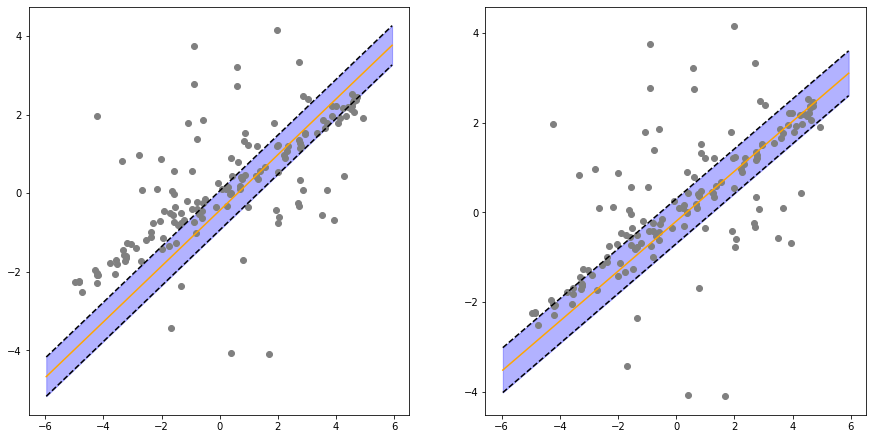
\includegraphics[width=\textwidth]{exercise_imgs/ex7-7.png}
			\end{block}
		\end{column}
	\end{columns}
\end{frame}

\begin{frame}{ Week 8: Transform invariant features }
	\begin{columns}
		\begin{column}{.45\textwidth}
			\begin{block}{Detected points}
			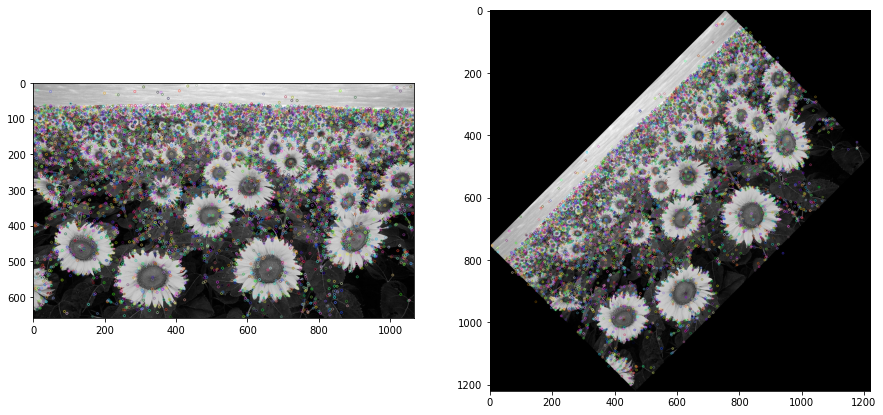
\includegraphics[width=\textwidth]{exercise_imgs/ex8-1.png}
			\end{block}
		\end{column}
		\begin{column}{.45\textwidth}
			\begin{block}{Matched detected points}
			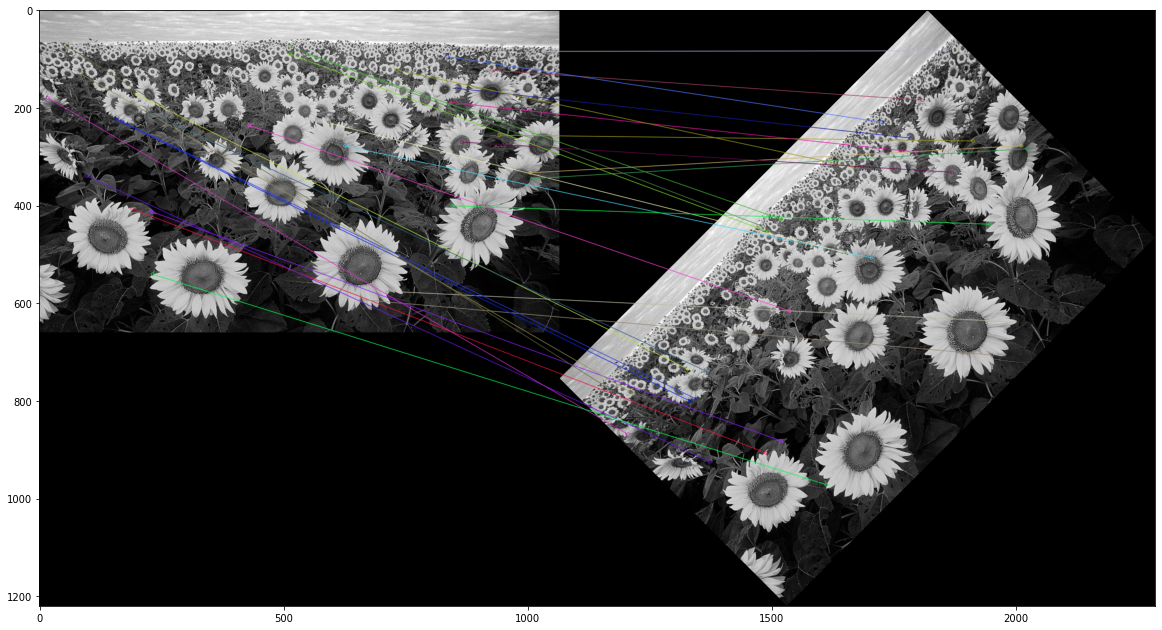
\includegraphics[width=\textwidth]{exercise_imgs/ex8-2.png}
			\end{block}
		\end{column}
	\end{columns}
\end{frame}

\begin{frame}{ Week 9: Geometry constrained feature matching }
	\begin{block}{Without and with Fest-8point regularization}
		\begin{center}
			\includegraphics[width=.5\textwidth]{exercise_imgs/ex9-4.png}
		\end{center}
	\end{block}
\end{frame}

\begin{frame}{ Week 10: Image stitching }
	\begin{columns}
		\begin{column}{.45\textwidth}
			\begin{block}{Warp of right image using hest}
			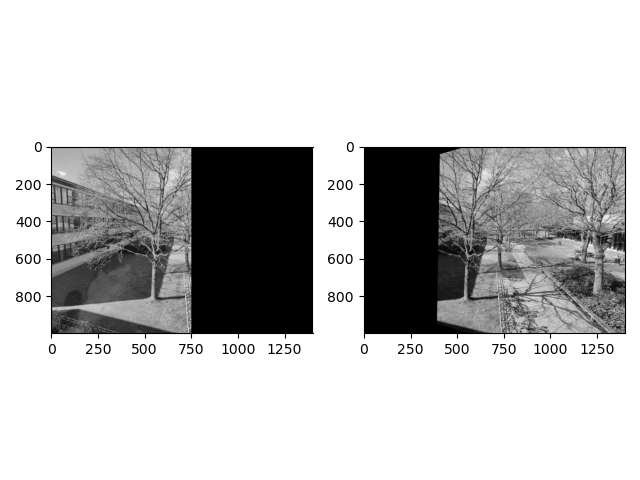
\includegraphics[width=\textwidth]{exercise_imgs/ex10-4.png}
			\end{block}
		\end{column}
		\begin{column}{.45\textwidth}
			\begin{block}{Stitched images}
			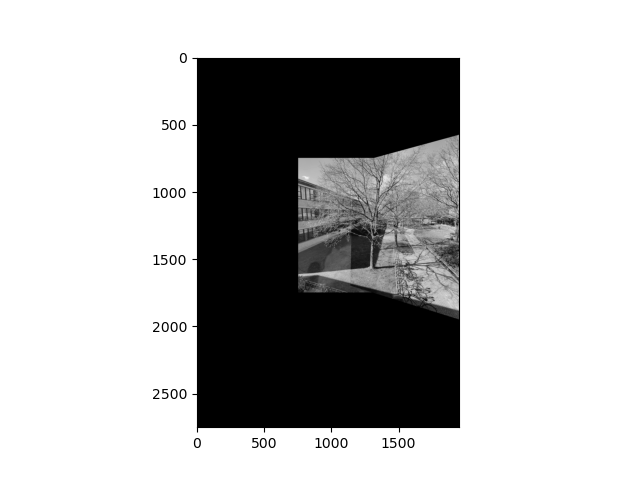
\includegraphics[width=\textwidth]{exercise_imgs/ex10-5.png}
			\end{block}
		\end{column}
	\end{columns}

\end{frame}

\begin{frame}{ Week 11-12: Motion estimation }
	\begin{columns}
		\begin{column}{.65\textwidth}
			\begin{block}{Common matched points}
			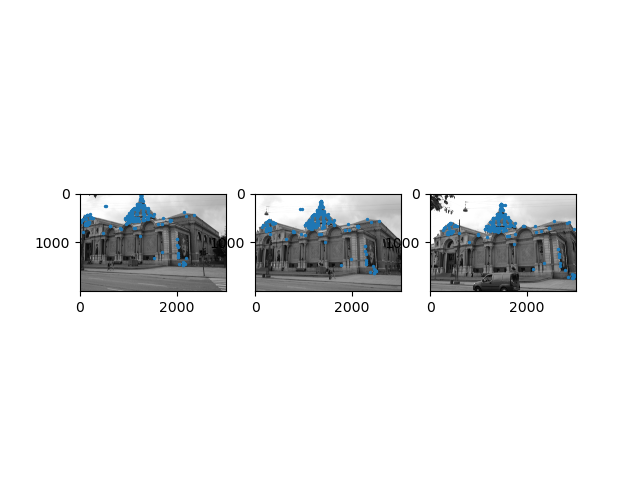
\includegraphics[width=\textwidth]{exercise_imgs/ex11-3.png}
			\end{block}
		\end{column}
		\begin{column}{.3\textwidth}
			\begin{block}{Common points in 3d space}
				\begin{center}
					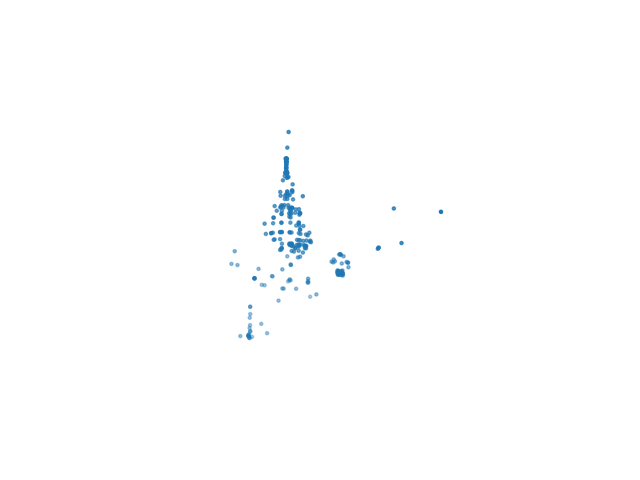
\includegraphics[width=1.5\textwidth]{exercise_imgs/ex11-4.png}
				\end{center}
			\end{block}
		\end{column}
	\end{columns}
\end{frame}

\begin{frame}{ Week 13: Structured light }
	\begin{columns}
		\begin{column}{.3\textwidth}
			\begin{block}{Rectified}
			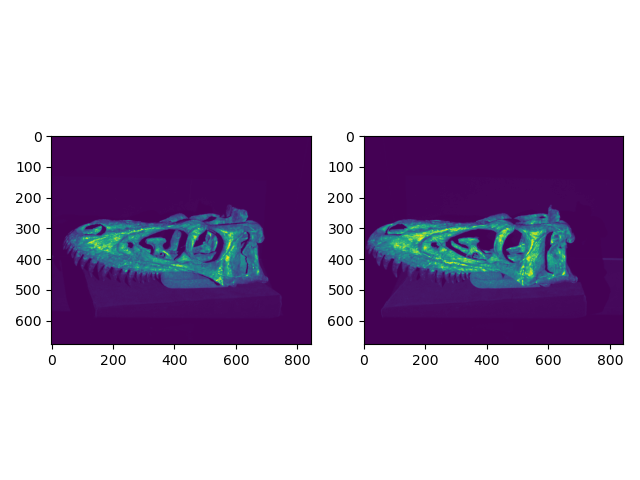
\includegraphics[width=\textwidth]{exercise_imgs/ex13-1.png}
			\end{block}
		\end{column}
		\begin{column}{.3\textwidth}
			\begin{block}{Phase}
				\begin{center}
					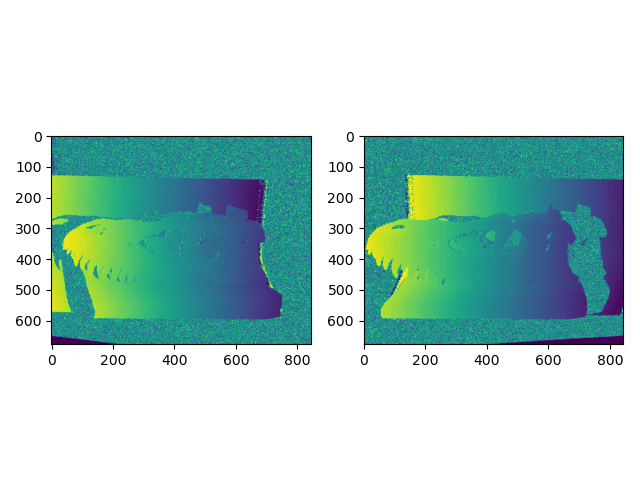
\includegraphics[width=\textwidth]{exercise_imgs/ex13-2.png}
				\end{center}
			\end{block}
		\end{column}
		\begin{column}{.3\textwidth}
			\begin{block}{Disparity}
				\begin{center}
					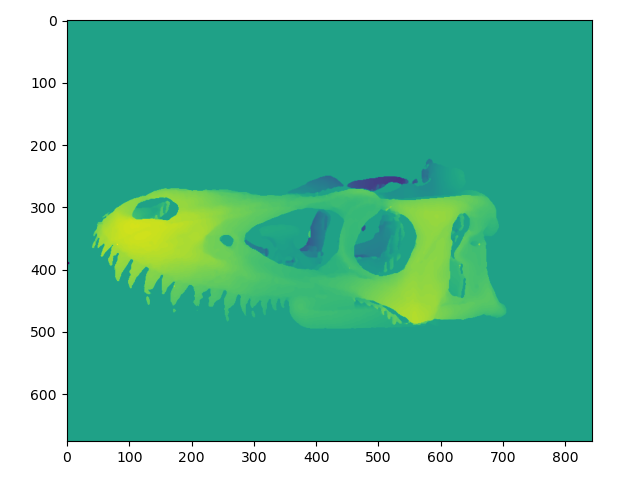
\includegraphics[width=\textwidth]{exercise_imgs/ex13-4.png}
				\end{center}
			\end{block}
		\end{column}
	\end{columns}
\end{frame}
\end{document}
